\documentclass[11pt]{beamer}
\usetheme{Madrid}
\usepackage[utf8]{inputenc}
\usepackage{amsmath}
\usepackage{amsfonts}
\usepackage{amssymb}
\usepackage{tikz}
\usepackage{pgf}
\usepackage{wrapfig,lipsum,booktabs, multicol, subfigure, empheq, ulem, multirow}
\usepackage{cancel}
\usetikzlibrary{positioning, fit, calc, arrows, matrix}   
\tikzset{block/.style={draw, thick, text width=2cm ,minimum height=3.3cm, align=center},   
line/.style={-latex}     
}  

\tikzstyle{int}=[draw, fill=blue!20, minimum size=2em]
\tikzstyle{init} = [pin edge={to-,thin,black}]
\tikzstyle{init2} = [pin edge={from-,thin,black}]

\author{Birol Yüceoğlu}
\title{DA 507 - Optimization and Modeling}
\subtitle{Lecture 2 \\ Linear Programming: Examples \\ Integer Programming: Examples}
%\setbeamercovered{transparent} 
%\setbeamertemplate{navigation symbols}{} 
%\logo{} 
\institute{Migros T.A.Ş.} 
%\date{} 
%\subject{byuceoglu@migros.com.tr} 
\begin{document}

\begin{frame}
\titlepage
\end{frame}

%\begin{frame}
%\tableofcontents
%\end{frame}

\section{DA507-Week1-2.txt}

\begin{frame}
\frametitle{Agenda}
\begin{itemize}
\item \textbf{Linear Programming: Examples}
\item \textbf{Integer Programming: Examples}
\item Solving LPs: Graphical Solution Method
\item Solving LPs: Simplex Algorithm
\end{itemize}

\end{frame}


\begin{frame}
\frametitle{Introduction to Optimization Modeling}
\begin{itemize}
\item Prescriptive models “prescribes” behavior for an organization that will enables it to best meet its goals.  Components of this model include
\begin{itemize}
\item objective function(s),
\item decision variables,
\item constraints.
\end{itemize}
\item An optimization model seeks to find values of the decision variables that optimize (maximize or minimize) an objective function among the set of all values for the decision variables that satisfy the given constraints.
\end{itemize}

\end{frame}



\begin{frame}
\frametitle{Introduction to Optimization Modeling (Eli Daisy)}
\begin{itemize}
\item<1-> Eli Daisy produces the drug Wozac in huge batches by heating a chemical mixture in a pressurized container.  Each time a batch is produced, a different amount of Wozac is produced. The amount produced is the process yield  (measured in pounds).
\item<1-> Daisy is interested in understanding the factors that influence the yield of Wozac production process.
\end{itemize}
\end{frame}

\begin{frame}
\frametitle{Introduction to Optimization Modeling (Eli Daisy)}

We seek to maximize the yield for the production process. To maximize the process yield we need to find the values of V, P, T, A, B, and C that make the yield equation (below) as large as possible.
\begin{equation}
  \begin{array}{l}
Yield = 300 + 0.8V +0.01P + 0.06T + 0.001TP - 0.01T^2 – 0.001P^2 \notag\\
+ 11.7A + 9.4B + 16.4C + 19A*B + 11.4AC – 9.6BC
\end{array}
\end{equation}
\pause

\begin{itemize}
\item Objective function
\item A function to be maximized or minimized
\item Only certain values of the decision variables are possible; such restrictions on the decision variable values are called constraints
\end{itemize}
\end{frame}
\begin{frame}
\frametitle{Introduction to Optimization Modeling (Eli Daisy)}
A descriptive model to determine the following factors influence yield:
\begin{itemize}
\item Container volume in liters (V)
\item Container pressure in milliliters (P)
\item Container pressure in degrees centigrade (T)
\item Chemical composition of the processed mixture (A, B, C)
\end{itemize}
\pause
\begin{itemize}
\item Volume must be between 1 and 5 liters ($1 \leq V \leq 5$),
\item Pressure must be between 200 and 400 milliliters ($200 \leq P \leq 400$),
\item Temperature must be between 100 and 200 degrees centigrade ($100 \leq T \leq 200$),
\item Mixture must be made up entirely of A, B, and C ($A+B+C = 1$),
\item For the drug to perform properly, only  half the mixture at most can be product A ($A \leq 0.5$).
\end{itemize}
\end{frame}

\begin{frame}
\frametitle{Eli Daisy}
Any specification of the decision variables (i.e. volume, pressure, etc..) that satisfies all the model’s constraints is said to be in the \textit{feasible region}.  
For example, a \textit{feasible solution} is \\
V = 2, P = 300, T = 150, A = 0.4,  B = 0.3, C = 0.3\\
\mbox{ } \\

Using some optimization software, it can be determined that the \textit{optimal solution}, i.e. a specification of the decision variables that satisfy the constraints and produces the maximum yield,  to its model is
\\V = 5, P = 200, T = 100, A = 0.294, B = 0, C = 0.706 with yield 209.384

\end{frame}

\begin{frame}
\frametitle{Linear Programming}
\begin{itemize}[<+->]
\item Linear programming is a powerful tool developed in 1930s and 1940s.
\item We aim to optimize a linear function subject to linear constraints.
\item Can be efficiently solved (in polynomial time).
\item Assumptions of linear programming:
\begin{itemize}
\item Proportionality: If a variable is doubled, its contribution to the objective function and the constraints is also doubled (no setup cost, savings)
\item Additivity: The total cost or the contribution to the constraints is the sum of individual contributions (no interaction or substitution)
\item Divisibility: Decision variables are continuous (no integrality required)
\item Deterministic: The coefficient of the cost and the constraints are known apriori (or are approximated)
\end{itemize}
\item Some of these requirements can be relaxed/modeled by using integer programming (at the expense of computation time).
\end{itemize}

\end{frame}

\begin{frame}
\frametitle{What is Linear Programming (LP)?}
\begin{itemize}
\item Linear programming (LP) is concerned with the optimization of a linear function over a set of linear constraints or restrictions.
\item In 1947, George B. Dantzig worked on a logistical supply “program.” Everything, in fact, started with Dantzig’s work.
\item However even before Dantzig, in 1939, Kantorovich worked on this problem and found a solution with organization and planning.
\item Since Kantorovich’s work is not known until 1959, the solution method proposed by Dantzig now enjoys a wide acceptance. This solution method is known as the simplex method.
\end{itemize}

\end{frame}

\begin{frame}
\frametitle{The Carpenter’s Problem}
\begin{itemize}
\item A carpenter tries to solve a weekly production planning problem to maximize profit.  He solely makes tables and chairs, and sells all tables and chairs at a market place.
\item Both chairs and tables require the same type of raw material.  The raw material availability is only 50 units per week.
\begin{itemize}
\item one chair requires 1 unit of the raw material;
\item one table requires 2 units of the raw material.
\end{itemize}
\item The carpenter can work at most 40 hours every week. It takes 2 hours to make a chair while it takes only an hour to make a table.
\item The cost of a chair is 100 TL and it sells for 120 TL; the cost of a table is 130 TL and it sells for 145 TL.
\end{itemize}

\end{frame}


\begin{frame}
\frametitle{The Carpenter’s Problem}
\begin{itemize}
\item Develop a profit maximizing mathematical model which takes into account both the raw material and labor hour constraints:
\begin{itemize}
\item Define your decision variables.
\item Write down the objective function.
\item Write down the constraints and the domain of the decision variables.
\end{itemize}
\end{itemize}

\end{frame}


\begin{frame}
\frametitle{The Carpenter’s Problem}
\begin{itemize}
\item Define your decision variables.
\item Write down the objective function.
\item Write down the constraints and the domain of the decision variables.
\end{itemize}
\pause  
\begin{itemize}
\item $x_1$ = number of chairs produced/sold each week
\item $x_2$ = number of table produced/sold each week
\end{itemize}
\pause  
\begin{align}
\displaystyle maximize \mbox{ } & (120-100)x_1 + (145-130)x_2, \label{carpenter:objective} \\
% 
\mbox{subject to }&2 x_1 + x_2  \leq 40, & \mbox{(labor)}  \label{carpenter:labor}\\
&x_1 + 2 x_2  \leq 50, & \mbox{(material)}  \label{carpenter:material}\\
& x_1, x_2 \geq 0. & \mbox{(domain)} \label{carpenter:domain}
\end{align}

\end{frame}

\begin{frame}
%------------------------------------------
\begin{wrapfigure}{r}{0.5\textwidth}
  \vspace{-40pt}
\begin{center}
\includegraphics[width=0.48\textwidth]{carpenter_c1.pdf}
\end{center}
\end{wrapfigure} 
%------------------------------------------
{Consider the labor constraint only: 

$2 x_1 + x_2  \leq 40$
\begin{itemize}
\item How many chairs can you produce if you do not produce any tables?

\begin{itemize}
\item 20
\end{itemize}
\item How many tables can you produce if you do not produce any chairs?

\begin{itemize}
\item 40
\end{itemize}
\item How many tables can you produce if you produce 10 chairs?

\begin{itemize}
\item 40
\end{itemize}
\end{itemize}}
%------------------------------------------
\end{frame}

\begin{frame}

\begin{multicols}{2}[\columnsep2em] 
Consider the labor constraint only: 

$2 x_1 + x_2  \leq 40$
\begin{itemize}
\item<1-> How many chairs can you produce if you do not produce any tables?
\pause
\begin{itemize}
\item 20
\end{itemize}
\item<2-> How many tables can you produce if you do not produce any chairs?
\pause
\begin{itemize}
\item 40
\end{itemize}
\item<3-> How many tables can you produce if you produce 10 chairs?
\pause
\begin{itemize}
\item 20
\end{itemize}
\end{itemize}
\columnbreak
\pause
\includegraphics[width=\linewidth]{carpenter_c1.pdf}%


\end{multicols}

\end{frame}


\begin{frame}

\begin{multicols}{2}[\columnsep2em] 
Consider the material constraint only: 

$x_1 + 2x_2  \leq 50$
\begin{itemize}
\item<1-> How many chairs can you produce if you do not produce any tables?
\pause
\begin{itemize}
\item 50
\end{itemize}
\item<2-> How many tables can you produce if you do not produce any chairs?
\pause
\begin{itemize}
\item 20
\end{itemize}
\item<3-> How many tables can you produce if you produce 10 chairs?
\pause
\begin{itemize}
\item 20
\end{itemize}
\end{itemize}
\columnbreak
\pause
\includegraphics[width=\linewidth]{carpenter_c2.pdf}%


\end{multicols}

\end{frame}

\begin{frame}
\begin{figure}
\centering
\begin{subfigure}
  \centering
  \includegraphics[width=.45\textwidth]{carpenter_1.pdf}
\end{subfigure}% \pause
\begin{subfigure}
  \centering
  \includegraphics[width=.45\textwidth]{carpenter_2.pdf}
\end{subfigure}
\caption{Feasible region.}
\end{figure}

\end{frame}
\begin{frame}{The Carpenter's Problem (New Constraint)}
The carpenter realizes that he needs a special glue to make the products and that every week he only has enough for 28 chairs and tables. He uses the same amount of glue for a chair and a table.

How do we modify the model?
\begin{itemize}
\item Decision variables
\pause
\begin{itemize}
\item No change
\end{itemize}
\item Constraints
\begin{itemize}
\item $x_1 + x_2 \leq 28$
\end{itemize}
\item Feasible region
\begin{itemize}
\item Changes
\end{itemize}
\item Profit
\begin{itemize}
\item Changes
\end{itemize}
\end{itemize}

\end{frame}
\begin{frame}
\begin{figure}
\centering
\includegraphics[scale=0.4]{carpenter_3.pdf}
\end{figure}
\end{frame}

\begin{frame}{The Carpenter's Problem (New Product)}
The carpenter can also produce stools with a profit of 5\$. Each stool uses 0.5 hours of labor and 0.5 unit of material.
\pause
\begin{itemize}
\item $x_1$ = number of chairs produced/sold each week
\item $x_2$ = number of table produced/sold each week
\item $x_3$ = number of stools produced/sold each week
\end{itemize}
\pause  
\begin{align}
\displaystyle maximize \mbox{ } & 20x_1 + 15x_2 + 5 x_3, \label{carpenter2:objective} \\
% 
\mbox{subject to }&2 x_1 + x_2 + 0.5x_3  \leq 40, & \mbox{(labor)}  \label{carpenter2:labor}\\
&x_1 + 2 x_2 +0.5x_3 \leq 50, & \mbox{(material)}  \label{carpenter2:material}\\
& x_1, x_2, x_3 \geq 0. & \mbox{(domain)} \label{carpenter2:domain}
\end{align}
\end{frame}

\begin{frame}
\frametitle{GUROBI}
\end{frame}
\begin{frame}
\frametitle{The Dream Diet Meal Plan}
\begin{itemize}
\item My dream diet requires that all the food I eat come from one of the four “basic food groups”
\item At present, the following four foods are available for consumption: brownies, chocolate ice cream, cola and strawberry cheesecake.
\item Each brownie costs 50 cents, each scoop of icecream costs 20 cents ,each bottle of cola costs 30 cents and each piece of cheesecake costs 80 cents.
\item Each day, I must ingest at least 500 calories, 6 oz of chocolate, 10 oz of sugar and 6 oz of fat. The nutritional content per unit of each food is shown in the table below. Formulate a linear programming model that can be used to satisfy my daily requirements at minimum cost.
\end{itemize}

\end{frame}


\begin{frame}
\frametitle{The Dream Diet Meal Plan}

\begin{table}
\centering
\begin{tabular}{l|llll}
Type of food & Calories & Chocolate & Sugar  & Fat  \\ 
\hline
\hline
Brownie & 400 & 3 & 2 & 2  \\ 
Ice cream (1 scoop) & 200 & 2 & 2 & 4  \\ 
Coke (1 bottle) & 150 & 0 & 4 & 1  \\ 
Cheesecake (1 piece) & 500 & 0 & 4 & 5  \\
\end{tabular}
\end{table}

Decision variables:
\begin{itemize}
\item $x_1$ = brownie pieces		
\item $x_2$ = scoops of ice cream
\item $x_3$ = bottles of coke	
\item $x_4$ = cheesecake pieces
\end{itemize}
\end{frame}


\begin{frame}
\frametitle{The Dream Diet Meal Plan}
\pause
\begin{align}
\displaystyle minimize \mbox{ } & 50x_1 + 20x_2 + 30 x_3 + 80 x_4, \label{diet:objective} \\
% 
\mbox{subject to }&400 x_1 + 200 x_2 + 150x_3 + 500 x_4 \geq 500, & \mbox{(calories)}  \label{diet:calories}\\
& 3x_1 + 2 x_2  \geq 6, & \mbox{(sugar)}  \label{diet:sugar}\\
& 2x_1 + 2 x_2 + 4x_3 + 4 x_4 \geq 10, & \mbox{(chocolate)}  \label{diet:chocolate}\\
& 2x_1 + 2 x_2 + x_3 + 5x_4 \geq 8, & \mbox{(fat)}  \label{diet:fat}\\
& x_1, x_2, x_3,x_4 \geq 0. & \mbox{(domain)} \label{diet:domain}
\end{align}

\end{frame}





\begin{frame}
\frametitle{A Multi-plant Production Model}
\begin{itemize}
\item There are two factories A and B. Each factory makes two products, standard and deluxe:
\begin{itemize}
\item a unit of standard gives a profit contribution of 10 TL;
\item a unit of deluxe gives a profit contribution of 15 TL.
\end{itemize}
\item Each factory uses two processes: polishing and grinding.
\begin{itemize}
\item Factory A has a grinding capacity of 80 hours and polishing capacity for 60 hours.
\item Factory B has a grinding capacity of 60 hours and polishing capacity for 75 hours.
\end{itemize}
\item Grinding a standard product in factory A takes 4 hours, while a deluxe product takes 2 hours. The same processing times in factory B are 5 and 3 hours, respectively.
\item Polishing a standard product in factory A takes 2 hours, while a deluxe product takes 5 hours. The same processing times in factory B are 5 and 6 hours, respectively.
\end{itemize}

\end{frame}


\begin{frame}
\frametitle{A Multi-Plant Production Model}
\begin{itemize}
\item Each unit of each product uses 4 kg. of a raw material. Of 120 kg raw material, the company has allocated
\begin{itemize}
\item 75 kg to factory A, and
\item 45 kg  to factory B.
\end{itemize}
%\item The demand for standard product is 8 and the demand for the deluxe product is 6.
\item Formulate a mathematical model to determine the production amounts of each product in the factories such that the overall profit is maximized.
\end{itemize}

Decision variables:
\begin{itemize}
\item $x_{SA}$ = the amount of standard product produced at plant A
\item $x_{DA}, x_{SB}, x_{DB}$ are defined similarly for products deluxe and plant B
\end{itemize}
\end{frame}


\begin{frame}
\frametitle{A Multi-Plant Production Model}


\pause
\begin{align}
\displaystyle minimize \mbox{ } & 10(x_{SA} + x_{SB}) + 15(x_{DA} + x_{DB}), \label{multi:objective} \\
% 
%\mbox{subject to }&x_{SA} + x_{SB} \leq 8, & \mbox{(demand (S))}  \label{multi:demand}\\
%& x_{DA} + x_{DB} \leq 6, & \mbox{(demand (D))}  \label{multi:demand1}\\
\mbox{subject to }& 4(x_{SA} + x_{DA}) \leq 75, & \mbox{(material (A))}  \label{multi:material}\\
& 4x_{SA} + 2x_{DA} \leq 80, & \mbox{(grinding (A))}  \label{multi:grinding}\\
& 2x_{SA} + 5x_{DA} \leq 60, & \mbox{(polishing (A))}  \label{multi:polishing}\\
& 4(x_{SB} + x_{DB}) \leq 45, & \mbox{(material (B))}  \label{multi:material1}\\
& 5x_{SB} + 3x_{DB} \leq 60, & \mbox{(grinding (B))}  \label{multi:grinding1}\\
& 5x_{SB} + 6x_{DB} \leq 75, & \mbox{(polishing (B))}  \label{multi:polishing1}\\
& x_{SA}, x_{DA}, x_{SB}, x_{DB} \geq 0. & \mbox{(domain)} \label{multi:domain}
\end{align}
\end{frame}

\begin{frame}
\frametitle{A Multi-Plant Production Model}


\begin{align}
\displaystyle maximize \mbox{ } & 10x_{SA} + 15x_{DA}, \label{multi1:objective} \\
% 
%\mbox{subject to }&x_{SA} + x_{SB} \leq 8, & \mbox{(demand (S))}  \label{multi:demand}\\
%& x_{DA} + x_{DB} \leq 6, & \mbox{(demand (D))}  \label{multi:demand1}\\
\mbox{subject to }& 4(x_{SA} + x_{DA}) \leq 75, & \mbox{(material (A))}  \label{multi1:material}\\
& 4x_{SA} + 2x_{DA} \leq 80, & \mbox{(grinding (A))}  \label{multi1:grinding}\\
& 2x_{SA} + 5x_{DA} \leq 60, & \mbox{(polishing (A))}  \label{multi1:polishing}\\
& x_{SA}, x_{DA} \geq 0. & \mbox{(domain)} \label{multi1:domain}
\end{align}
\pause
\begin{align}
\displaystyle maximize \mbox{ } & 10 x_{SB} + 15 x_{DB}, \label{multi2:objective} \\
% 
%\mbox{subject to }&x_{SA} + x_{SB} \leq 8, & \mbox{(demand (S))}  \label{multi:demand}\\
%& x_{DA} + x_{DB} \leq 6, & \mbox{(demand (D))}  \label{multi:demand1}\\
\mbox{subject to }& 4(x_{SB} + x_{DB}) \leq 45, & \mbox{(material (B))}  \label{multi2:material1}\\
& 5x_{SB} + 3x_{DB} \leq 60, & \mbox{(grinding (B))}  \label{multi2:grinding1}\\
& 5x_{SB} + 6x_{DB} \leq 75, & \mbox{(polishing (B))}  \label{multi2:polishing1}\\
& x_{SA}, x_{DA}, x_{SB}, x_{DB} \geq 0. & \mbox{(domain)} \label{multi2:domain}
\end{align}
\end{frame}
\begin{frame}
\frametitle{A Multi-Plant Production Model}
% Table generated by Excel2LaTeX from sheet 'Sheet1'
\begin{table}[htbp]
  \centering
  \caption{Optimal solution for plants A and B.}
    \begin{tabular}{lrrr}
          & \multicolumn{1}{l}{Plant A} & \multicolumn{1}{l}{Plant B} & \multicolumn{1}{l}{Total} \\
    Standart & 11.25 & 0     & 11.25 \\
    Deluxe & 7.5   & 11.25 & 18.75 \\
    \hline
    Profit & 225   & 168.75 & 393.75 \\
    \end{tabular}%
  \label{tab:addlabel}%
\end{table}%

\end{frame}

\begin{frame}
\frametitle{A Multi-Plant Production Model}
\begin{itemize}
\item Each unit of each product uses 4 kg. of a raw material. \textbf{The company has 120 kg of raw material available.} \sout{Of 120 kg raw material, the company has allocated}
\begin{itemize}
\item \sout{75 kg to factory A, and}
\item \sout{45 kg  to factory B.}
\end{itemize}
%\item The demand for standard product is 8 and the demand for the deluxe product is 6.
\item Formulate a mathematical model to determine the production amounts of each product in the factories such that the overall profit is maximized.
\end{itemize}

Decision variables:
\begin{itemize}
\item $x_{SA}$ = the amount of standard product produced at plant A
\item $x_{DA}, x_{SB}, x_{DB}$ are defined similarly for products deluxe and plant B
\end{itemize}
\end{frame}

\begin{frame}
\frametitle{A Multi-Plant Production Model}


\pause
\begin{align}
\displaystyle maximize \mbox{ } & 10(x_{SA} + x_{SB}) + 15(x_{DA} + x_{DB}), \label{multi3:objective} \\
% 
%\mbox{subject to }&x_{SA} + x_{SB} \leq 8, & \mbox{(demand (S))}  \label{multi:demand}\\
%& x_{DA} + x_{DB} \leq 6, & \mbox{(demand (D))}  \label{multi:demand1}\\
\mbox{subject to }& 4x_{SA} + 2x_{DA} \leq 80, & \mbox{(grinding (A))}  \label{multi3:grinding}\\
& 2x_{SA} + 5x_{DA} \leq 60, & \mbox{(polishing (A))}  \label{multi3:polishing}\\
& 5x_{SB} + 3x_{DB} \leq 60, & \mbox{(grinding (B))}  \label{multi3:grinding1}\\
& 5x_{SB} + 6x_{DB} \leq 75, & \mbox{(polishing (B))}  \label{multi3:polishing1}\\
& 4x_{SB} + 4x_{DB} +5x_{SB} + 6x_{DB} \leq 120, & \mbox{(material)}  \label{multi3:material1}\\
& x_{SA}, x_{DA}, x_{SB}, x_{DB} \geq 0. & \mbox{(domain)} \label{multi3:domain}
\end{align}
\end{frame}

\begin{frame}
\frametitle{A Multi-Plant Production Model}
% Table generated by Excel2LaTeX from sheet 'Sheet1'
\begin{table}[htbp]
  \centering
  \caption{Optimal solutions for fixed and free allocation scenarios.}
    \begin{tabular}{lrrrcrrr}
    & \multicolumn{3}{c}{Fixed Allocation} & &\multicolumn{3}{c}{Free Allocation}  \\
          & \multicolumn{1}{l}{Plant A} & \multicolumn{1}{l}{Plant B} & \multicolumn{1}{l}{Total} & \multirow{4}[0]{*}{vs.} & \multicolumn{1}{l}{Plant A} & \multicolumn{1}{l}{Plant B} & \multicolumn{1}{l}{Total} \\
    Standart & 11.25 & 0     & 11.25 &       & 9.167 & 0     & 9.167 \\
    Deluxe & 7.5   & 11.25 & 18.75 &       & 8.33  & 12.5  & 20.83 \\
    Profit & 225   & 168.75 & 393.75 &       &       &       & 404.167 \\
    \end{tabular}%
\end{table}%

\end{frame}
\begin{frame}{GUROBI}

\end{frame}
\begin{frame}
\frametitle{Transportation Problem}
\begin{itemize}
\item The Brazilian coffee company processes coffee beans into coffee at 3 plants. The coffee is then shipped every week to 7 warehouses in major cities for retail, distribution, and exporting.
\item It is desired to find the production-shipping pattern $x_{ij}$ from plant $i$ to warehouse $j, i = 1,\ldots ,3, j = 1,\ldots,7$, that minimizes the overall shipping cost.
\item Suppose that the unit shipping cost from plant $i$ to warehouse $j$ is $c_{ij}$. Further suppose that the production capacity at plant $i$ is $a_i$ and that the demand at warehouse $j$ is $b_j$.
\item  This the well-known transportation problem.
\end{itemize}

\end{frame}


\begin{frame}
\frametitle{Transportation Problem}
\begin{figure}
\centering
\includegraphics[scale = 0.5]{transportation.png}
\end{figure}
\end{frame}
%
%\begin{frame}
%\frametitle{Transportation Problem}
%\begin{figure}[h]
%  \footnotesize
%  \centering
%  \begin{tikzpicture}[
%    % type of arrow head
%    &gt;=stealth',
%    % keep arrow head from touching the surface
%    shorten &gt;= 1pt,
%    % automatic node positioning
%    auto,
%    % 
%    node distance=2cm,
%    % line thickness
%    semithick,
%    bend angle=10,
%    graybox/.style = {draw=gray!20, fill=gray!20, rounded corners},
%    line/.style = {draw=black, thick},
%    box/.style = {circle, draw=blue!50, fill=blue!20, minimum size=7mm}
%    ]
% 
% 
%    \coordinate (S1) at (-3cm, 1.5cm);
%    \coordinate (S2) at (-3cm, 0.5cm);
%    \coordinate (S3) at (-3cm, -0.5cm);
%
%    \coordinate (M1) at (0cm, 3.5cm);
%    \coordinate (M2) at (0cm, 2.5cm);
%    \coordinate (M3) at (0cm, 1.5cm);
%    \coordinate (M4) at (0cm,  .5cm);
%    \coordinate (M5) at (0cm,- .5cm);
%    \coordinate (M6) at (0cm,-1.5cm);
%    \coordinate (M7) at (0cm,-2.5cm);
% 
% 
%     % nodes
%    \node (Sbox1) [box] at (S1) {1};
%    \node (Sbox2) [box] at (S2) {2};
%    \node (Sbox3) [box] at (S3) {3};
%     
%    \node (Mbox1) [box] at (M1) {$1$};
%    \node (Mbox2) [box] at (M2) {$2$};
%    \node (Mbox3) [box] at (M3) {$3$};
%    \node (Mbox4) [box] at (M4) {$4$};
%    \node (Mbox5) [box] at (M5) {$5$};
%    \node (Mbox6) [box] at (M6) {$6$};
%    \node (Mbox7) [box] at (M7) {$7$};
%          
%
% 
%    % edges
% 
%    \path[line] (Sbox1) -- node [above] {} (Mbox1);
%    \path[line] (Sbox2) -- node [above] {} (Mbox1);
%    \path[line] (Sbox3) -- node [above] {} (Mbox1);
% 
%    \path[line] (Sbox1) -- node [above] {} (Mbox2);
%    \path[line] (Sbox2) -- node [above] {} (Mbox2);
%    \path[line] (Sbox3) -- node [above] {} (Mbox2);
%
%    \path[line] (Sbox1) -- node [above] {} (Mbox3);
%    \path[line] (Sbox2) -- node [above] {} (Mbox3);
%    \path[line] (Sbox3) -- node [above] {} (Mbox3);
%    
%	\path[line] (Sbox1) -- node [above] {} (Mbox4);
%    \path[line] (Sbox2) -- node [above] {} (Mbox4);
%    \path[line] (Sbox3) -- node [above] {} (Mbox4);
%    
%	\path[line] (Sbox1) -- node [above] {} (Mbox5);
%    \path[line] (Sbox2) -- node [above] {} (Mbox5);
%    \path[line] (Sbox3) -- node [above] {} (Mbox5);
%    
%    \path[line] (Sbox1) -- node [above] {} (Mbox6);
%    \path[line] (Sbox2) -- node [above] {} (Mbox6);
%    \path[line] (Sbox3) -- node [above] {} (Mbox6);
%    
%    \path[line] (Sbox1) -- node [above] {} (Mbox7);
%    \path[line] (Sbox2) -- node [above] {} (Mbox7);
%    \path[line] (Sbox3) -- node [above] {} (Mbox7);        
%   \end{tikzpicture}
% \end{figure}
%\end{frame}



\begin{frame}
\frametitle{Transportation Problem}
$x_{ij}$ = the amount sent from plant $i$ to warehouse $j$.
\pause
\begin{align}
\displaystyle minimize \mbox{ } & \sum_{i=1}^{3} \sum_{j=1}^{7} c_{ij} x_{ij}, \label{transport:objective} \\
% 
\mbox{subject to }&\sum_{j=1}^{7} x_{ij} \leq a_i, & \forall i \in\{1,2,3\} \mbox{(capacity)}  \label{transport:capacity}\\
&\sum_{i=1}^{3} x_{ij} \geq b_j, & \forall j \in\{1,\ldots,7\} \mbox{(demand)}  \label{transport:demand}\\
& x_{ij} \geq 0, &\forall i \in\{1,2,3\} \forall j \in\{1,\ldots,7\} \mbox{(domain)} \label{transport:domain}
\end{align}

\end{frame}


\begin{frame}
\frametitle{Transportation Problem}
\begin{itemize}
\item A company ships their products from three different plants (one in LA, one in Atlanta, and one in New York City) to four regions of the United States (East, Midwest, South, West).
\item Each plant has a capacity on how many products can be sent out, and each region has a demand of products they must receive.
\item There is a different transportation cost between each plant, or each city, and each region.
\item The company wants to determine how many products each plant should ship to each region in order to minimize the total transportation cost.
\end{itemize}

\end{frame}


\begin{frame}
\frametitle{Transportation Problem}
\begin{itemize}
\item Decision variables:
\begin{itemize}
\item The amount to ship from each plant to each region
\end{itemize}
\item Constraints:
\begin{itemize}
\item Demand: the total number of products received by a region (from each plant) is greater than or equal to its demand
\item Capacity: the total number of products shipped from a plant (to each region) is less than or equal to its capacity
\end{itemize}
\item Objective function:
\begin{itemize}
\item Minimize the total transportation costs
\end{itemize}
\end{itemize}

\end{frame}


\begin{frame}
\frametitle{Transportation Problem (Solver)}

\end{frame}

\begin{frame}
\frametitle{Airplane refueling (Adler, 1996)}
\begin{itemize}
\item Trans Global Airlines (TGA) wants to optimize its purchases of jet fuel at the cities it serves around the world.
\item Since the fuel efficiency of an airplane is related to its weight, an airplane carrying more fuel than needed to reach its destination will waste fuel.
\item This fact suggests that a plane should take off with just enough fuel to reach its next destination.
\item However, since fuel prices vary from city to city, a policy of minimal fuel purchases may be more costly than filling the plane to capacity at the inexpensive cities.
\item You are tasked with minimizing the fuel related costs while respecting the safety.
\end{itemize}

\end{frame}


\begin{frame}
\frametitle{Airplane Refueling (Adler, 1996)}
\begin{itemize}
\item To illustrate TGA’s problem, consider an airplane that flies each day a so-called rotation that consists of the following four flight segments:
\item 	New York $\rightarrow$ Los Angeles $\rightarrow$ San Francisco $\rightarrow$ Seattle
\item 	Upon its arrival in New York, the airplane repeats the rotation.
\end{itemize}
% Table generated by Excel2LaTeX from sheet 'Sheet1'
\begin{table}[htbp]
  \centering
    \begin{tabular}{llrrlr}
    \multicolumn{1}{c}{Departure}  & \multicolumn{1}{c}{Arrival} & \multicolumn{1}{c}{A} & \multicolumn{1}{c}{B} & \multicolumn{1}{c}{C}     & \multicolumn{1}{c}{D} \\ 
    \multicolumn{1}{c}{City}  & \multicolumn{1}{c}{City} & \multicolumn{3}{c}{(gallons)}  & \multicolumn{1}{c}{(cents)} \\
    \hline
    \hline
    New York & Los Angeles & 23    & 33    & $2.90 + 0.40G$ & 82 \\
    Los Angeles & San Francisco & 8     & 19    & $1.60 + 0.05G$ & 75 \\
    San Francisco & Seattle & 19    & 33    & $4.75 +0.25G$ & 77 \\
    Seattle & New York & 25    & 33    & $1.75+0.45G$ & 89 \\
    \end{tabular}%
\end{table}%
A: Minimal fuel level at take-off

B: Maximal fuel level at take-off

C: Fuel consumption as a function of take-off weight $G$ 

D: Price per gallon fuel at the departure city

\end{frame}


\begin{frame}
\frametitle{Airplane Refueling (Adler, 1996)}

\pause
$x_{i}$: the amount of fuel purchased at city $i$ ($i = NY,LA,SF,SE$)

$a_{i}$: the amount of fuel the plane has at arrival to city $i$ 

$d_{i}$: the amount of fuel the plane has at departure from city $i$ 

\pause
\begin{align}
\displaystyle minimize \mbox{ } & 82 x_{NY} + 75 x_{LA} + 77x_{SF} + 89 x_{SE}, \label{refuelling:objective} \\
% 
\mbox{subject to }&23 \leq d_{NY} \leq 33, & \mbox{(fuel level)}  \label{refuelling:level1}\\
%&8 \leq d_{LA} \leq 19, & \mbox{(fuel level)}  \label{refuelling:level2}\\
%&19 \leq d_{SF} \leq 33, & \mbox{(fuel level)}  \label{refuelling:level3}\\
%&25 \leq d_{SE} \leq 33, & \mbox{(fuel level)}  \label{refuelling:level4}\\
& a_{NY} + x_{NY} = d_{NY},& \mbox{(balance)}  \label{refuelling:balance1}\\
& d_{NY} - 2.9 - 0.4d_{NY} = a_{LA},& \mbox{(consumption)} \label{refuelling:consumption}\\
&x_{i}, a_{,}, d_{i} \geq 0, & \forall i \in cities \mbox{ (domain)} \label{refuelling:domain}
\end{align}

Constraints~\eqref{refuelling:level1}-\eqref{refuelling:consumption} should be written for each city.
\end{frame}

\begin{frame}

\begin{figure}
\centering
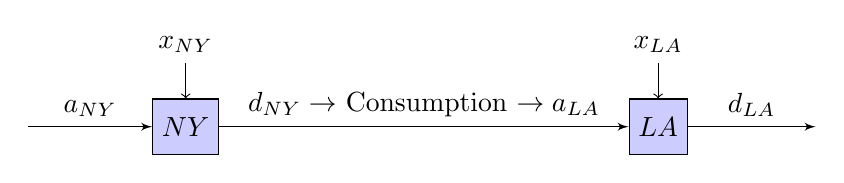
\begin{tikzpicture}[node distance=2.5cm,auto,>=latex']
    \node [int, pin={[init]above:$x_{NY}$}] (a) {$NY$};
    \node (b) [left of=a,node distance=2cm, coordinate] {a};
    \node [int, pin={[init]above:$x_{LA}$}] (c) [right of=a, node distance = 6cm] {$LA$};
    \node [coordinate] (end) [right of=c, node distance=2cm]{};
    \path[->] (b) edge node {$a_{NY}$} (a);
    \path[->] (a) edge node {$d_{NY} \rightarrow$ Consumption  $\rightarrow a_{LA}$} (c);
    \draw[->] (c) edge node {$d_{LA}$} (end) ;

\end{tikzpicture}

\end{figure}
\end{frame}
\begin{frame}
\frametitle{Cutting Stock Problem}
\begin{itemize}
\item A manufacturer of metal sheets produces rolls of standard fixed width $w$ and of length of 10 meters.
\item A large order is placed by a customer who needs sheets of width $w$ and varying lengths such as 1.5, 2.5, 3.0, and 4.0. Demand for each is 10, 12, 15 and 7 sheets, respectively.
\item The manufacturer would like to cut the standard rolls in such a way as to satisfy the order and to minimize the waste. Since scrap pieces are useless to the manufacturer, the objective is to minimize the number of rolls needed to satisfy the order (or total scrapped metal sheets).
\end{itemize}
\end{frame}

\begin{frame}
\frametitle{Cutting Stock Problem}
Given a standard sheet of 10 meters, there are many ways of cutting it. We consider the following five patterns, where each number corresponds to the number of sheets of length 1.5, 2.5, 3.0, and 4.0.
\[
a_{1} = 
\left[
\begin{array}{c}
3 \\
2 \\
0\\
0\\
\end{array}\right] ,
a_{2} = 
\left[
\begin{array}{c}
0 \\
4 \\
0\\
0\\
\end{array}\right] ,
a_{3} = 
\left[
\begin{array}{c}
0 \\
0 \\
3\\
0\\
\end{array}\right] ,
a_{4} = 
\left[
\begin{array}{c}
0 \\
0 \\
2 \\
1 \\
\end{array}\right] ,
a_{5} = 
\left[
\begin{array}{c}
1 \\
1 \\
0\\
1\\
\end{array}\right]\]

Note that when the patterns are not given (i.e. any pattern respecting the length of the sheet is possible) the problem becomes notoriously difficult.
\end{frame}


\begin{frame}
\frametitle{Cutting Stock Problem}
$x_{1}$ = the number of sheets cut using pattern $a_{1}$. $x_{2},\ldots,x_{5}$ are defined analogously.
\pause
\begin{align}
\displaystyle minimize \mbox{ } & \sum_{i=1}^{5}  x_{i}, \label{stock:objective} \\
% 
\mbox{subject to }&3x_{1} + x_{5} \geq 10, & \mbox{(demand (1.5))}  \label{stock:demand1}\\
&2x_{1} + 4x_{2} + x_{5} \geq 12, &  \mbox{(demand (2.5))}  \label{stock:demand2}\\
&3x_{3} + 2x_{4} \geq 15, & \mbox{(demand (3.0))}  \label{stock:demand3}\\
&x_{4} + x_{5} \geq 7, &  \mbox{(demand (4.0))}  \label{stock:demand4}\\
& x_{i} \geq 0, &\forall i \in\{1,\ldots,5\}  \mbox{(domain)} \label{stock:domain}
\end{align}
\end{frame}


\begin{frame}
\frametitle{Steel Production Planning (Adler, 1996)}
\begin{itemize}
\item Consider the production planning problem of the National Steel Corporation (NSC), which produces a special-purpose steel that is used in the aircraft and aerospace industries. The marketing department of NSC has received orders for 2400, 2200, 2700, and 2500 tons of steel during each of the next four months: NSC can meet these demands by producing the steel by drawing from its inventory, or by any combination thereof.
\item The production costs per ton of steel during each of the next four months are projected to be $7400, $7500, $7600, and $7800. Because of these inflationary costs, it might be advantageous for NSC to produce more steel than it is needs in a given month and store the excess, although production capacity can never exceed 4000 tons in any month. All production takes place at the beginning of the month, and immediately thereafter the demand is met. The remaining steel is then stored in inventory at a cost of \$120/ton for each month that it remains there.
\end{itemize}

\end{frame}


\begin{frame}
\frametitle{Steel Production Planning (Adler, 1996)}
\begin{itemize}
\item If the production level is increased or decreased from one month to the next, the company incurs a cost for implementing these changes. Specifically, for each ton of increased or decreased production over the previous month, the cost is \$50. The production of the first month, however, is exempt from this cost.
\item The inventory at the beginning of the first month is 1000 tons of steel and the inventory level at the end of the fourth month should be at least 1500 tons.
\item Formulate a production planning problem for NSC that will minimize the total cost over the next four months.
\end{itemize}

\end{frame}

%
%\begin{frame}
%\frametitle{Steel Production Planning (Adler, 1996)}
%
%\begin{figure}
%\centering
%\begin{tikzpicture}[node distance=2.5cm,auto,>=latex']
%    \node [int, pin={[init]above:$p_1$}] (a) {Period 1};
%    \node [int, pin={[init2]below:$d_1$}] (a) {Period 1};
%    \node (b) [left of=a,node distance=2cm, coordinate] {a};
%    \node [int, pin={[init]above:$p_2$}] (c) [right of=a, node distance = 6cm] {Period 2};
%    \node [coordinate] (end) [right of=c, node distance=2cm]{};
%    \path[->] (b) edge node {$1000$} (a);
%    \path[->] (a) edge node {$d_{1} \rightarrow$ Consumption  $\rightarrow a_{LA}$} (c);
%    \draw[->] (c) edge node {$d_{LA}$} (end) ;
%
%\end{tikzpicture}
%
%\end{figure}
%
%\end{frame}

\begin{frame}
\frametitle{Steel Production Planning (Adler, 1996)}
$p_{i}$: steel production at period $i = 1,\ldots,4$.

$i_{i}$: inventory at the end of period $i = 0,1,\ldots,4$.

$y_{i}$: increase in production at period $i = 2,3,4$.

$z_{i}$: decrease in production at period $i = 2,3,4$.

\pause

\[ Cost = 7400p_1 + 7500p_2 + 7600p_3 + 7800p_4 + 120 \sum_{i=1}^{3} i_i + 50 \sum_{i=2}^{4} (z_i+y_i) \]
\pause
\begin{align}
\displaystyle minimize \mbox{ } & Cost, \label{steel:objective} \\
\mbox{subject to }&p_1 + i_0 \geq 2400, & \mbox{(demand)}  \label{steel:demand}\\
&p_2 + i_1 \geq 2200, & \mbox{(demand)}  \label{steel:demand2}\\
&p_3 + i_2 \geq 2700, & \mbox{(demand)}  \label{steel:demand3}\\
&p_4 + i_3 \geq 2500, & \mbox{(demand)}  \label{steel:demand4}
\end{align}
\end{frame}

\begin{frame}
\frametitle{Steel Production Planning (Adler, 1996)}

\begin{align}
&p_1 + i_0 -2400 = i_1, & \mbox{(balance)}  \label{steel:balance}\\
&p_2 + i_1 -2400 = i_2, & \mbox{(balance)}  \label{steel:balance2}\\
&p_3 + i_2 -2400 = i_3, & \mbox{(balance)}  \label{steel:balance3}\\
&p_4 + i_3 -2400 = i_4, & \mbox{(balance)}  \label{steel:balance4}\\
&i_0 = 1000, i_4 \geq 1500, & \mbox{(inventory)}  \label{steel:inventory}\\
&p_i \leq 4000, & \forall i \in \{1,2,3,4\} \mbox{(production)}  \label{steel:production}\\
&p_i,i_1 \geq 0, & \mbox{(domain)}  \label{steel:domain}
\end{align}
\pause
Demand constraints from the previous slide are not necessary as they are covered by the balance constraints.
\end{frame}

\begin{frame}
\frametitle{Steel Production Planning (Adler, 1996)}
Let us see how we can incorporate production level change constraints.
\pause
\begin{align}
&y_2 \geq p_2 - p_1, z_2 \geq p_1 - p_2, & \mbox{(change)}  \label{steel:change}\\
&y_3 \geq p_3 - p_2, z_3 \geq p_2 - p_3, & \mbox{(change)}  \label{steel:change2}\\
&y_4 \geq p_4 - p_3, z_4 \geq p_3 - p_3, & \mbox{(change)}  \label{steel:change3}\\
& y_i, z_i \geq 0, & \mbox{(domain)} \label{steel:domain2}
\end{align}
\end{frame}

\begin{frame}
\frametitle{Tanker scheduling}
A shipline company requires a fleet of ships to service requirements for carrying cargo between six cities. There are four specific routes that must be served daily with the given number of ships.

\includegraphics[scale=.5]{img0007.png}

\end{frame}


\begin{frame}
\frametitle{Tanker scheduling}
All cargo are compatible, and therefore only one type of ship is needed. It takes one day to off-load and one day to on-load each ship. How many ships must the shipline company purchase?
\includegraphics[scale=0.5]{img0008.png}

\end{frame}

\begin{frame}
\frametitle{Tanker scheduling}
$x_{ij}$: the number of ships coming off of route $i$ and assigned to route $j$.

$c_{ij}$: the number of ships required to have a continuous daily flow (number of days for route $i$ + number of days to travel from end of route $i$ to the beginning of route $j$ + 2 days for off\&on-loading ($c_{ij}$ is a parameter).
\pause
Example:
$x_{11}$: the number of ships coming off of route Dhahran-New York and is assigned to route Dhahran-New York (the ship travels from Dhahran to New York, off\&on-loads, travels back to Dhahran to start the second journey. Note that this includes one journey (from Dhahran to New York) and the preparation for the start of the second journey (the ship is relocated to Dhahran to start the second journey, which in this case is Dhahran-New York)

$c_{11} = 17 + 2 + 17 = 36$
\end{frame}

\begin{frame}
\frametitle{Tanker scheduling}
\begin{align}
\displaystyle minimize \mbox{ } & 36 x_{11} + 32x_{12} + 33 x_{13}+19x_{14} + \ldots, \label{tanker:objective} \\
\mbox{subject to }&\sum_{j=1}^{4} x_{ij} = b_i, & \mbox{(out flow)}  \label{tanker:outflow}\\
&\sum_{i=1}^{4} x_{ij} = b_j, & \mbox{(in flow)}  \label{tanker:inflow}\\
&x_{ij} \geq 0, & \forall i,j  \mbox{(domain)}  \label{tanker:domain}
\end{align}

$b_1 = 3, b_2 = 2, b_3 = 1, b_4 = 1$


\pause
\fbox{\begin{minipage}{30em}
Note that this problem is slightly more involved than most of the content in the course. It is included to illustrate two points
\begin{itemize}
\item Decision variables are not always trivial to define.
\item Sometimes you do the modeling while defining your variables.
\end{itemize}
\end{minipage}}
\end{frame}


\begin{frame}{Integer Programming}
\begin{itemize}
\item<1-> Integer programming (also called integer linear programming, ILP) deals with a similar setting.
\item<2-> The objective function and the constraints are stated in the same fashion.
\item<3-> The domain constraint are replaced by integrality constraints.
\item<4-> Integer variables can be necessary to model real-life problems as you cannot sell half of something.
\item<5-> Integer (binary) variables are required to model various kinds of constraints as well.
\end{itemize}
\end{frame}

\begin{frame}
\frametitle{The Carpenter’s Problem}
\begin{itemize}
\item A carpenter tries to solve a weekly production planning problem to maximize profit.  He solely makes tables and chairs, and sells all tables and chairs at a market place.
\item Both chairs and tables require the same type of raw material.  The raw material availability is only 50 units per week.
\begin{itemize}
\item one chair requires 1 unit of the raw material;
\item one table requires 2 units of the raw material.
\end{itemize}
\item The carpenter can work at most 40 hours every week. It takes 2 hours to make a chair while it takes only an hour to make a table.
\item The cost of a chair is 100 TL and it sells for 120 TL; the cost of a table is 130 TL and it sells for 145 TL.
\end{itemize}

\pause
\fbox{\begin{minipage}{30em}
What if we can only sell complete chairs or tables?
\end{minipage}}
\end{frame}


\begin{frame}
\frametitle{The Carpenter’s Problem}
\begin{itemize}
\item $x_1$ = number of chairs produced/sold each week
\item $x_2$ = number of table produced/sold each week
\end{itemize}
\pause  
\begin{align}
\displaystyle maximize \mbox{ } & (120-100)x_1 + (145-130)x_2, \label{carpenter1:objective} \\
% 
\mbox{subject to }&2 x_1 + x_2  \leq 40, & \mbox{(labor)}  \label{carpenter1:labor}\\
&x_1 + 2 x_2  \leq 50, & \mbox{(material)}  \label{carpenter1:material}\\
& \cancel{x_1, x_2 \geq 0 }\mbox{ } x_1, x_2 \in \mathbb{Z^+}. & \mbox{(domain)} \label{carpenter1:domain}
\end{align}

\end{frame}

\begin{frame}
\begin{figure}
\centering
\begin{subfigure}
  \centering
  \includegraphics[width=.42\textwidth]{carpenter_2.pdf}
\end{subfigure}% \pause
\begin{subfigure}
  \centering
  \includegraphics[width=.35\textwidth]{Carpenter_ip.pdf}
\end{subfigure}
\caption{Feasible region for an IP consists of a set of points (rhs).}
\end{figure}

\end{frame}


\begin{frame}
\frametitle{The Carpenter's Problem}
If the customer wants to buy a set (one table and two chairs), the selling price is 360 TL. You can only sell an integer number of sets ( no such restriction on chairs or tables). Modify the mathematical model accordingly to reflect this new product option and the profit to be made from this option.

$x_3$ = number of sets produced/sold each week

\pause  
\begin{align}
\displaystyle maximize \mbox{ } & 20 x_1 + 15x_2 + 55x_3, \label{carpenter23:objective} \\
% 
\mbox{subject to }&2 x_1 + x_2  + 5 x_3\leq 40, & \mbox{(labor)}  \label{carpenter23:labor}\\
&x_1 + 2 x_2  + 4x_3\leq 50, & \mbox{(material)}  \label{carpenter23:material}\\
&x_1, x_2 \geq 0, x_3 \in \mathbb{Z^+}. & \mbox{(domain)} \label{carpenter23:domain}
\end{align}

You can mix different types of variables as long as the objective function and the constraints are linear.
\end{frame}

\begin{frame}
\frametitle{The Carpenter's Problem}
The carpenter has a fixed cost of 50 TL for producing chairs any week, and a fixed cost of 40 TL for producing tables. You do not incur the cost if you do not produce that item.
Do you need additional decision variables? If so, how could you define the new variables?
How does your model change?

\pause
\begin{equation}\nonumber
    y_{1} =
    \begin{cases}
      1, & \text{if the carpenter produces chairs,} \\
      0, & \text{otherwise.} \\
    \end{cases}
  \end{equation}\begin{equation}\nonumber
    y_{2} =
    \begin{cases}
      1, & \text{if the carpenter produces tables,} \\
      0, & \text{otherwise.} \\
    \end{cases}
  \end{equation}

The variables introduced here are called \textit{binary} variables. They are useful to model such conditions in integer programming.
  
\end{frame}

\begin{frame}
\frametitle{The Carpenter's Problem}
The carpenter has a fixed cost of 50 TL for producing chairs any week, and a fixed cost of 40 TL for producing tables. You do not incur the cost if you do not produce that item.
Do you need additional decision variables? If so, how could you define the new variables?
How does your model change?

\pause
  
\begin{align}
\displaystyle maximize \mbox{ } & 20x_1 + 15x_2 - 50 y_1 - 40 y_2, \label{carpenter3:objective} \\
% 
\mbox{subject to }&2 x_1 + x_2  \leq 40, & \mbox{(labor)}  \label{carpenter3:labor}\\
&x_1 + 2 x_2  \leq 50, & \mbox{(material)}  \label{carpenter3:material}\\
& x_1 \leq M y_1, & \mbox{(fixed cost)}  \label{carpenter3:fixed1}\\
& x_2 \leq M y_2, & \mbox{(fixed cost)}  \label{carpenter3:fixed2}\\
& x_1, x_2 \geq 0, & \mbox{(domain)} \label{carpenter3:domain}\\
& y_1, y_2 \in \{0,1\}. & \mbox{(domain)} \label{carpenter3:domain2}
\end{align}
  
\end{frame}

\begin{frame}
\frametitle{The Carpenter's Problem}
If the carpenter can produce at least 5 chairs (or 5 tables), then the labor requirement for the chair (or the table) is halved. This is only valid for the additional items. If the carpenter produces 5 chairs and 3 tables only the labor requirement for the chairs are halved.

\pause
$x_1, x_3$ = number of chairs produced/sold each week at normal / reduced labor

$x_2, x_4$ = number of table produced/sold each week at normal / reduced labor
\pause
\begin{equation}\nonumber
    y_{1} =
    \begin{cases}
      1, & \text{if the carpenter produces at least 5 chairs,} \\
      0, & \text{otherwise.} \\
    \end{cases}
  \end{equation}\begin{equation}\nonumber
    y_{2} =
    \begin{cases}
      1, & \text{if the carpenter produces at least 5 tables,} \\
      0, & \text{otherwise.} \\
    \end{cases}
  \end{equation}
\end{frame}

\begin{frame}
\frametitle{The Carpenter's Problem}
If the carpenter can produce at least 5 chairs (or 5 tables), then the labor requirement for the chair (or the table) is halved. This is only valid for the additional items. If the carpenter produces 5 chairs and 3 tables only the labor requirement for the chairs are halved.
\begin{align}
\displaystyle maximize \mbox{ } & 20(x_1 + x_3) + 15(x_2+x_4), \label{carpenter4:objective} \\
% 
\mbox{subject to }&2 x_1 + x_2 +x_3 + 0.5x_4 \leq 40, & \mbox{(labor)}  \label{carpenter4:labor}\\
&x_1 + 2 x_2 \leq 50, & \mbox{(material)}  \label{carpenter4:material}\\
& x_3 \leq M y_1, x1 \geq 5 y_1 & \mbox{(econ. of scale)}  \label{carpenter4:fixed1}\\
& x_4 \leq M y_2, x2 \geq 5 y_2 & \mbox{(econ. of scale)}  \label{carpenter4:fixed2}\\
& x_1, x_2, x_3, x_4 \geq 0, & \mbox{(domain)} \label{carpenter4:domain}\\
& y_1, y_2 \in \{0,1\}. & \mbox{(domain)} \label{carpenter4:domain2}
\end{align}

\end{frame}


\begin{frame}
\frametitle{Examples: Discrete Inputs and Outputs}
\begin{itemize}
\item Inputs can only be added in increments of machine capacity/week.
\item Workforce scheduling
\item Fleet optimization
\item Investment optimization: portfolio selection
\item Knapsack problem
\begin{itemize}
\item IP with a single constraint
\end{itemize}
\end{itemize}
\end{frame}

\begin{frame}
\frametitle{Examples: Problems with Logical Conditions}
\begin{itemize}
\item For instance, in a product mix problem if product A is manufactured, then product B or C must be manufactured as well.
\begin{itemize}
\item A mixed integer problem is obtained by introducing additional integer variables and constraints.
\end{itemize}
\item Selecting a depot location from a number of candidate sites.
\item Selecting a project from a number of alternatives.
\end{itemize}
\end{frame}


\begin{frame}
\frametitle{Examples: Combinatorial Problems}
\begin{itemize}
\item Sequencing problems
\begin{itemize}
\item Very often, operations need to be carried out in some sequence. Modeling precedence relationships requires use of integer variables.
\begin{itemize}
\item Job shop scheduling problem.
\item Traveling salesman problem.
\end{itemize}
\end{itemize}

\item Allocation problems
\begin{itemize}
\item Transportation and assignment problems (special case).
\item Allocating tasks to machines (line balancing).
\item Quadratic assignment problem.
\item Airline crew scheduling.
\end{itemize}
\end{itemize}
\end{frame}



\begin{frame}
\frametitle{Do we need IP?}
Consider the following problem
  
\begin{align}
\displaystyle maximize \mbox{ } & x_1 + x_2, \label{iplp:objective} \\
% 
\mbox{subject to }&-2 x_1 + 2x_2  \geq 1, &  \label{iplp:c1}\\
&-8x_1 + 10 x_2  \leq 13, &   \label{iplp:c2}\\
& x_1, x_2 \geq 0. &  \label{iplp:domain}
\end{align}
 
  
\begin{itemize}
\item<1-> The LP optimal solution is x1=4 and x2=4.5.
\item<2-> What happens if we round continuous variables?
\pause
\begin{itemize}
\item $x_2 = 4$ ?
\item $x_2 = 5$ ?
\end{itemize}
\item<3-> The IP optimal solution is x1=1 and x2=2.
\item<4-> The variables represent liters of beer vs. number of airplanes.
\item<5-> In general, the round-off error is smaller when the variables take large values.
\end{itemize}
\end{frame}

\begin{frame}
\begin{figure}
\centering
\includegraphics[scale=0.4]{IP_example.pdf}
\end{figure}
\end{frame}


\end{document}
